\documentclass[parskip=full,11pt,twoside]{scrartcl}
\usepackage[utf8]{inputenc}


% section numbers in margins:
\renewcommand\sectionlinesformat[4]{\makebox[0pt][r]{#3}#4}

% header & footer
\usepackage{scrlayer-scrpage}
\lofoot{\today}
\refoot{\today}
\pagestyle{scrheadings}

\usepackage[sfdefault,light]{roboto}
\usepackage[T1]{fontenc}
\usepackage[german]{babel}
\usepackage[yyyymmdd]{datetime} % must be after babel
\renewcommand{\dateseparator}{-} % ISO8601 date format
\usepackage{hyperref}
\usepackage[nameinlink]{cleveref}
\crefname{figure}{Abb}{Abb}
\usepackage[section]{placeins}
\usepackage{xcolor}
\usepackage{graphicx}
\hypersetup{
	pdftitle={Pflichtenheft},
	bookmarks=true,
}
\usepackage{csquotes}

\usepackage{amsmath} % for $\text{}$
\newcommand\urlpart[2]{$\underbrace{\text{\texttt{#1}}}_{\text{#2}}$}

\usepackage{pflichtenheft}


\begin{titlepage}
\subject{Pflichtenheft}
\title{{\Huge \lambda urora}}
\subtitle{The Lambda Calculus IDE}


\author{Julia Patrusheva, Alexander von Heyden\\
Younis Bensalah, Max Nowak\\ 
Nikolai Polley, Randy Seng}

\end{titlepage}




\begin{document}
\maketitle
\newpage
\section{Einleitung}


\pagebreak
\section{Kriterien}
% Diese Section sollte kurz und knapp "für Manager" sein
% und auf eine Seite passen.

\subsection{Musskriterien}

%\criterium{Schnelle Weiterleitung Kurz- zu Lang-URL}{crt:fast}


\subsection{Wunschkriterien}

%Der Dienst bietet eine Seite \enquote{Über Uns},
%mit Informationen zum Betreiber.

\subsection{Abgrenzungskriterien}

%\criteriumNot{Keine Wahl Kurz-URL}{crt:no-choice}

%Ein Nutzer hat keine Möglichkeit die Auswahl einer Kurz-URL zu beeinflussen.

\pagebreak
%%%%%%%%%%%%%%
\section{Produkteinsatz}


\section{Produktumgebung}


%%%%%%%%%%%
\section{Funktionale Anforderungen}

%\functionality{Login-Möglichkeit auf Homepage}{fnc:login}
%\fulfills{crt:login}
%\fulfills{crt:github}

%Auf der Homepage \texttt{http://atu.rl/} sieht ein Besucher
%einen \enquote{Login via Facebook} Knopf.
%Weitere Knöpfe wie \enquote{Login via Github} sind möglich.
%Siehe \cref{fig:homepage}.



%%%%%%%%%%%
\section{Nicht-Funktionale Anforderungen}

%\nonFunctionality{Modernes Design}{nfc:design}

%Das Design soll modern und seriös wirken.



%%%%%%%%%%%
\section{Tests}

%\test{Betreiberinfos lesen}{tst:tmg}
%\tests{fnc:impressum-link}
%\tests{fnc:datenschutz-link}

%\teststep{Besucher \enquote{Jayne Cobb} ist auf der Homepage}
%{Er folgt dem Link mit dem Text \enquote{Datenschutz}}
%{Ein Text mit allen Datenschutzinformationen wird ihm angezeigt.}

%\teststep{}
%{Jayne folgt dem Link mit dem Text \enquote{Impressum}}
%{Ein Text mit Informationen des Betreibers wird ihm angezeigt.}

\section{Entwicklungsumgebung}

%%%%%%%%%%%%%
\pagebreak
\appendix

\section{Seitenentwürfe}

% made via https://gomockingbird.com/projects/mnf0cwf/4gXVnC

%\begin{figure}[hb]
%\fbox{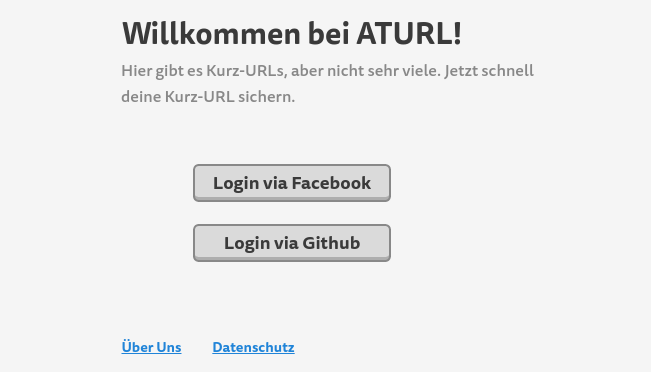
\includegraphics[width=\textwidth]{image/login.png}}
%\caption{\label{fig:homepage}
%Homepage mit Login-Funktion
%}
%\end{figure}


\section{Glossar}

%\textbf{Homepage}:
%Seite, die beim Besuchen der Betreiberdomain \emph{ohne Pfad} angezeigt wird. Auch %\enquote{Startseite}.


\end{document}
